\documentclass{beamer}
\usetheme[sectionpage = none,progressbar=frametitle, numbering = fraction]{metropolis}           % Use metropolis theme
\usepackage{color}
\usepackage{wrapfig}
\usepackage{graphicx}

\title{Desenvolvimento de plataforma robótica omnidirecional}
\date{18 de Dezembro, 2017}
\author{Emílio Dolgener Cantú \\ Orientador: Prof. Eduardo Perondi}
\institute{Universidade Federal do Rio Grande do Sul}
\begin{document}

% CAPA
\maketitle
% SUMÁRIO
\begin{frame}
  \frametitle{Sumário}
  \tableofcontents
\end{frame}
% O Q É O ROBÔ OMNIDIRECIONAL
\section{O Robô Omnidirecional}
\begin{frame}{Robô Omnidirecional}
  Holonomicidade: capacidade de se mover sem necessidade de reorientação.
  \begin{figure}[h]
    \centering
    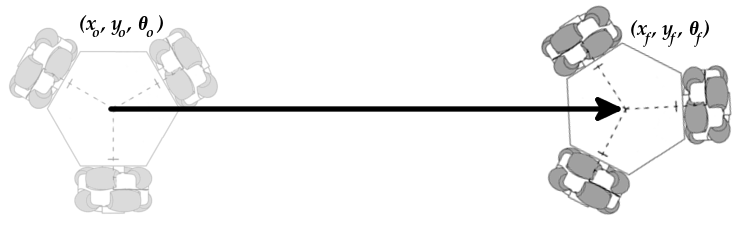
\includegraphics[width = \textwidth]{imagens/hibrida}
  \end{figure}
\end{frame}

\begin{frame}{Robô Omnidirecional}
  \emph{Omniwheel} (ou roda sueca):
  \begin{figure}[h]
    \centering
    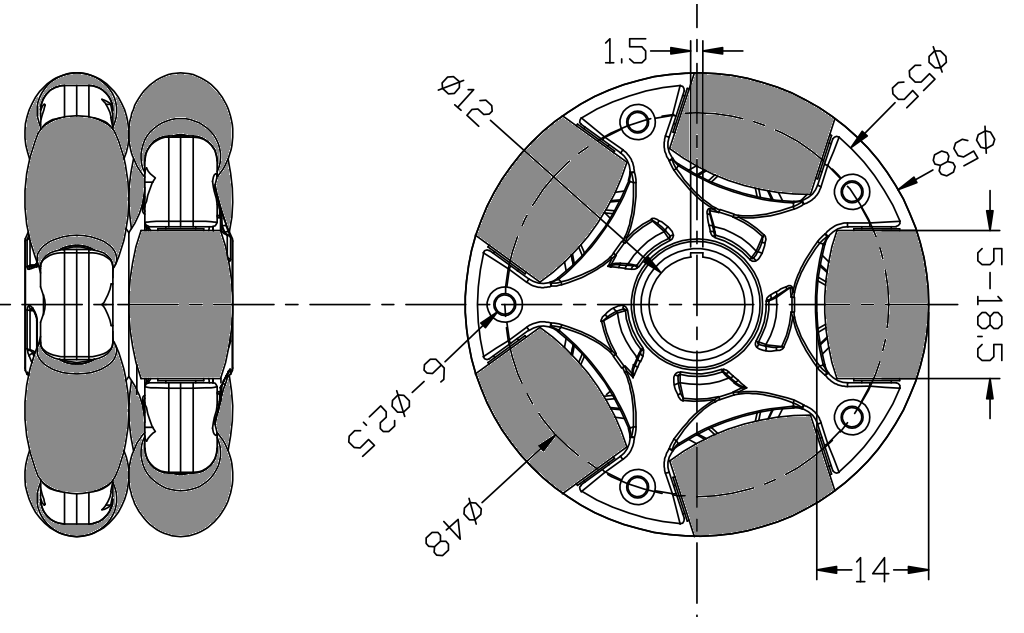
\includegraphics[width = 0.7\textwidth]{imagens/omniwheel}
  \end{figure}
\end{frame}
% REVISÃO BIBLIOGRÁFICA
% MOTIVAÇÃO
% OBJETIVOS

\section{Motivação e Objetivos}
\begin{frame}{Motivação}

 $\Delta x = v_x \Delta t $
  \begin{itemize}
    \item{Robótica: multi-disciplinaridade;}
    \item{Robótica móvel: aplicação na industria, visto que a maioria dos robôs são fixos no chão;}
    \item{Robô omnidirecional: transporte ágil de cargas pequenas em ambientes confinados;}
    \item{Interesse pessoal.}
  \end{itemize}
\end{frame}

\begin{frame}{Objetivos}
  \begin{tabular}{cl}
    \begin{tabular}{l}
      \parbox{0.6\linewidth}{%  change the parbox width as appropiate
      \begin{itemize}
        \item{Plataforma para trabalhos futuros;}
        \item[]{\textcolor{white}{blablablabalblablablablabal;}}
        \item[]{\textcolor{white}{Scuba diving is fun;}}
      \end{itemize}
      }
    \end{tabular}
    &
    \begin{tabular}{r}
      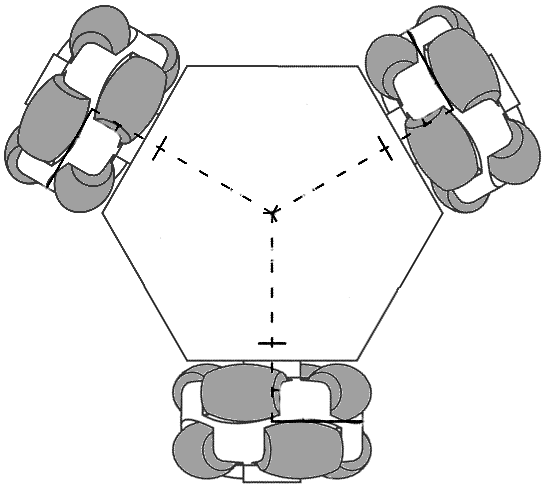
\includegraphics[width = 4 cm]{imagens/tomr_ritter_mod}
    \end{tabular} \\
  \end{tabular}
\end{frame}

\begin{frame}{Objetivos}
  \begin{tabular}{cl}
    \begin{tabular}{l}
      \parbox{0.6\linewidth}{%  change the parbox width as appropiate
      \begin{itemize}
        \item{\textcolor{gray}{lorem ipsum dolor sit amet;}}
        \item{blablablabalblablablablabal;}
        \item[]{\textcolor{white}{Scuba diving is fun;}}
      \end{itemize}
      }
    \end{tabular}
    &
    \begin{tabular}{r}
      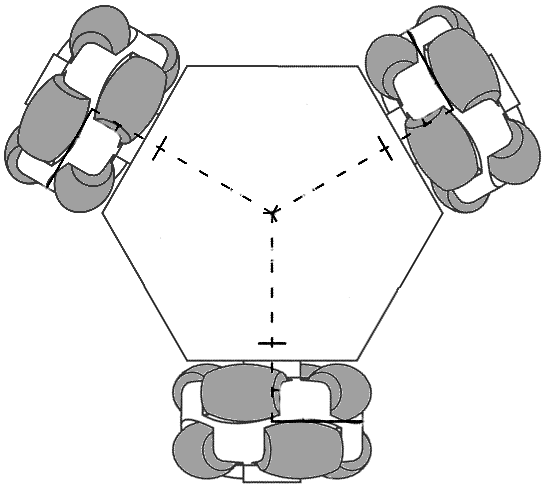
\includegraphics[width = 4 cm]{imagens/tomr_ritter_mod}
    \end{tabular} \\
  \end{tabular}
  \addtocounter{framenumber}{-1}
\end{frame}

\begin{frame}{Objetivos}
  \begin{tabular}{cl}
    \begin{tabular}{l}
      \parbox{0.6\linewidth}{%  change the parbox width as appropiate
      \begin{itemize}
        \item{\textcolor{gray}{lorem ipsum dolor sit amet;}}
        \item{\textcolor{gray}{blablablabalblablablablabal;}}
        \item{Plataforma para trabalhos futuros;}
      \end{itemize}
      }
    \end{tabular}
    &
    \begin{tabular}{r}
      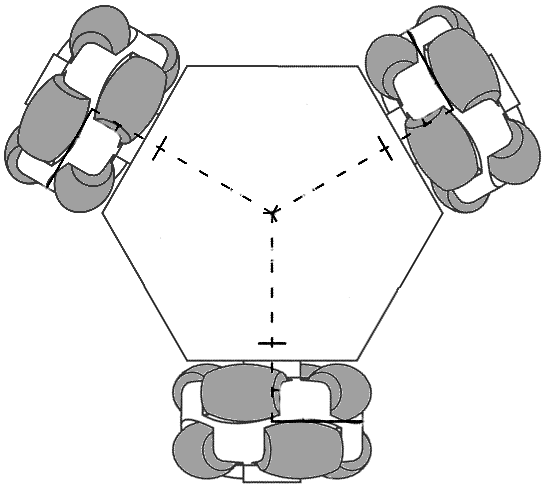
\includegraphics[width = 4 cm]{imagens/tomr_ritter_mod}
    \end{tabular} \\
  \end{tabular}
  \addtocounter{framenumber}{-1}
\end{frame}

\section{Desenvolvimento Teórico}
% MODELAGEM
\subsubsection{Modelagem}
%\subsubsection{Sistemas de Coordenadas}
\begin{frame}{Mundo - Robô}
  \begin{figure}[h]
    \centering
    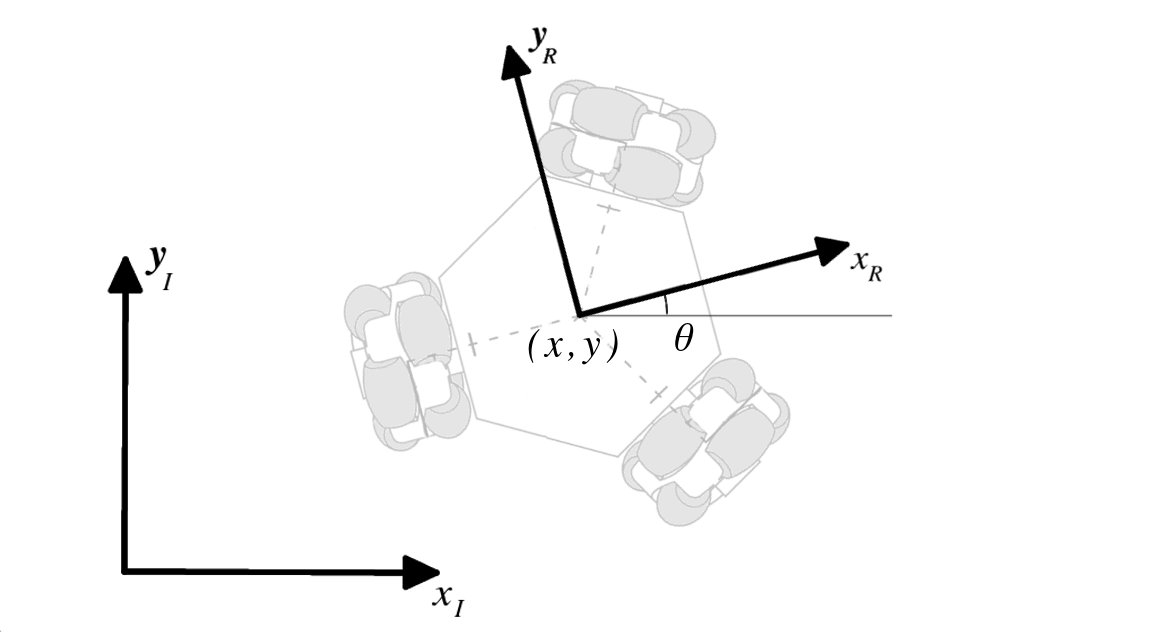
\includegraphics[width = 0.6\textwidth]{imagens/ref}
  \end{figure}

  \begin{equation}
    \begin{pmatrix}
      x_I \\
      y_I \\
      \theta
    \end{pmatrix}
    =
    \begin{pmatrix}
      cos \theta & -sen \theta & 0 \\
      sen\theta  &  cos \theta & 0 \\
      0          & 0          & 1
    \end{pmatrix}
    \begin{pmatrix}
      x_R \\
      y_R \\
      \theta
    \end{pmatrix}
    \label{eq:world_ref}
  \end{equation}

\end{frame}

\begin{frame}{Robô}
  Hello, world!
\end{frame}
% ODOMETRIA
\subsubsection{Odometria}
\begin{frame}{Odometria}
  Hello, world!
\end{frame}
% CONTROLE
\subsubsection{Controle}
%\subsubsection{de Velocidade}
\begin{frame}{Controle de Velocidade}
  Hello, world!
\end{frame}
%\subsubsection{de Posição}
\begin{frame}{Controle de Posição}
  Hello, world!
\end{frame}

\section{Protótipo}
% ESPECIFICAÇÃO DOS COMPONENTES
\subsubsection{Especificação dos Componentes}
\begin{frame}{Componentes}
  Hello, world!
\end{frame}

% FABRICAÇÃO + MONTAGEM
\subsubsection{Fabricação e Montagem}
\begin{frame}{Fabricação e Montagem}
  \begin{figure}[h]
    \centering
    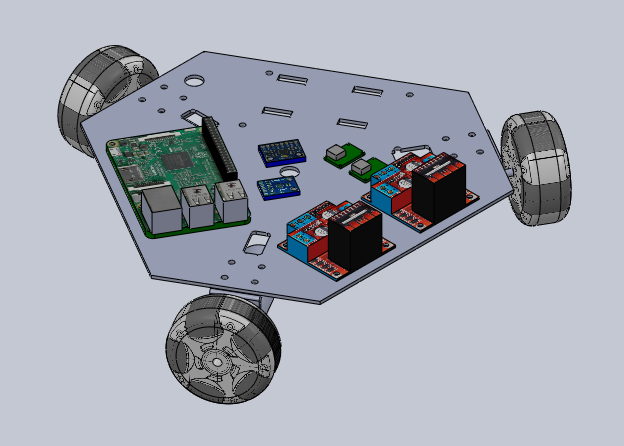
\includegraphics[width = 0.7\textwidth]{imagens/proto01}
  \end{figure}
\end{frame}
\begin{frame}
  \begin{figure}[h]
    \centering
    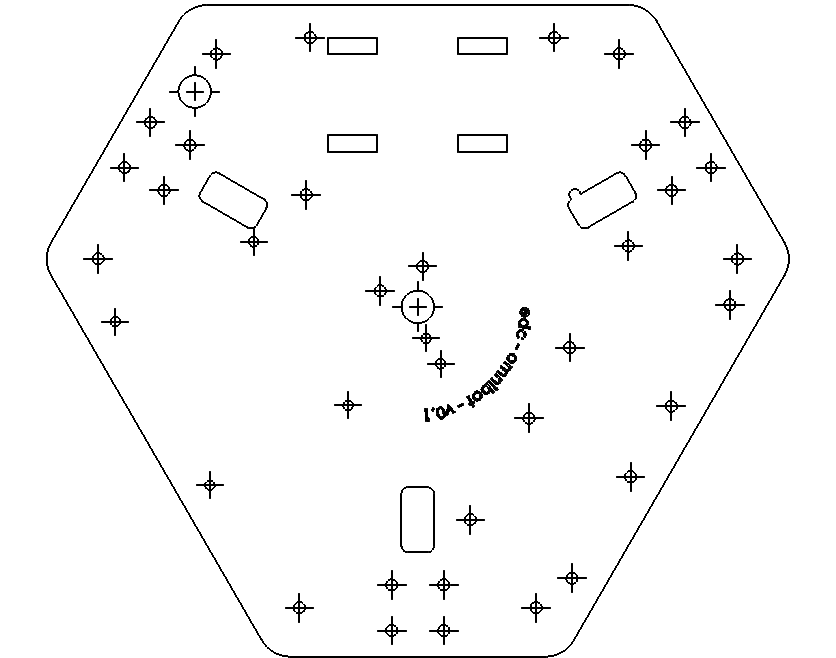
\includegraphics[width = 0.7\textwidth]{imagens/chassidxf}
  \end{figure}
\end{frame}
\begin{frame}{Fabricação e Montagem}
  \begin{figure}[h]
    \centering
    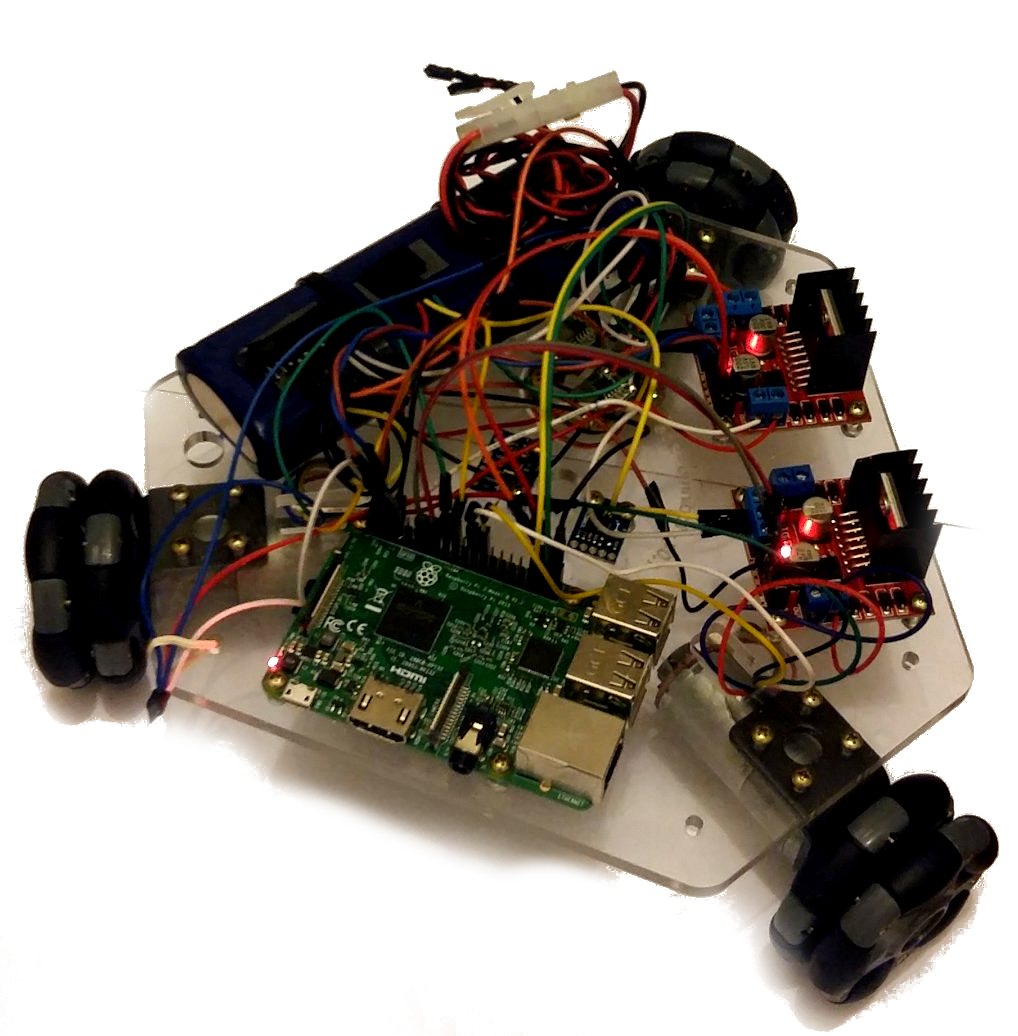
\includegraphics[width = 0.7\textwidth]{imagens/roboto}
  \end{figure}
  \addtocounter{framenumber}{-1}
\end{frame}

\section{Implementação do Software}
\begin{frame}{Implementação}
  Hello, world!
\end{frame}

\section{Resultados}
\begin{frame}{Resultados}
  Hello, world!
\end{frame}

\section{Conclusão e Trabalhos Futuros}
\begin{frame}{Resultados}
  Hello, world!
\end{frame}

\begin{frame}
  Muito obrigado!
\end{frame}

\end{document}
